\newpage
\chapter{Odstranění knihoven Cg toolkit, OpenGL z programu}
DicomPresenter využívá knihovnu OpenGL. Pomocí OpenGL jsou uloženy  MRI snímky v paměti počítače a dále jsou pomocí OpenGL vykreslovány na obrazovku. V programu byla dále použita knihovna Cg toolkit. Autor práce \cite{neskudla} obhajuje její použití tím, že v OpenGL se mu nedaří realizovat změnu jasu a kontrastu, a tak k tomuto používá Cg toolkit.

Tato kapitola má za cíl odpovědět na otázku, zda by bylo možné z programu odstranit knihovny OpenGL a Cg toolkit a dále, jaký dopad by to mělo na chod programu. V první části kapitoly je vysvětleno, co je to změna jasu a kontrastu. OpenGL, ani Cg toolkit nenabízejí pro změnu kontrastu předem naprogramované funkce a tak je třeba toto realizovat vlastním kódem. V druhé části kapitoly je pak zkoumán dopad absence OpenGL a Cg toolkit na plynulý běh programu.
% Změna kontrastu i posunování snímků jsou v DicomPresenteru řešeny real-time, tzn. program okamžitě reaguje na akce uživatele. Pro to, aby bylo možné odstranit knihovnu OpenGL z programu, musíme být schopni bez této knihovny realizovat obě úlohy alespoň 30x za sekundu. Pro odstranění knihovny Cg toolkit z programu musíme být schopni realizovat změnu jasu a kontrastu v OpenGL (případně pak i v C++ bez využití OpenGL).

\section{Jas  a kontrast}
Na začátku kapitoly si nejprve definujme, co jsou to jas a kontrast. V našem případě se můžeme omezit jen na černobílé snímky, protože výstupem MRI barevné snímky nejsou. Obrázek tedy můžeme chápat jako matici čísel mezi $0$ a $1$, kde sloupce, respektive řádky odpovídají souřadnicím bodu v obrázku:

\begin{equation}
 Im_{res_{x},res_{y}} =
 \begin{pmatrix}
  Im(1,1) & Im(1,2) & \cdots & Im(1,res_{x}) \\
  Im(2,1) & Im(2,2) & \cdots & Im(2,res_{x}) \\
  \vdots  & \vdots  & \ddots & \vdots  \\
  Im(res_{y},1) & Im(res_{y},2) & \cdots & Im(res_{y},res_{x})
 \end{pmatrix}
 Im(x,y) \in [0,1]
\end{equation}

Pro $ Im(x,y) = 0 $ vidíme pixel černý, pro $ Im(x,y) = 1 $ vidíme pixel bílý.

Jas a kontrast lze pak definovat\footnote{Jas je aritmetický průměr intenzit všech pixelů v obrázku. Kontrast snímku je roven směrodatné odchylce intenzit od jejich průměru.}\cite{wikipediaContrast}:

\begin{equation}
Brightness(Im) = \frac{1}{res_{x} \cdot res_{y}}\sum_{\substack{0 \leq x \leq res_{x} \\ 0 \leq y \leq res_{y}}} Im(x,y)
\end{equation}
\begin{equation}
Contrast(Im) = \sqrt{\frac{1}{res_{x} \cdot res_{y}}\sum_{\substack{ 0 \leq x \leq res_{x} \\ 0 \leq y \leq res_{y} }}(Im_{x,y}-Brightness(Im))^2}
\end{equation}

Pro změnu jasu a kontrastu snímku se pak v počítačových programech používají následující dvě funkce:

\begin{equation} Im(x,y) \longmapsto Im(x,y) + c_{brightness} \end{equation}
\begin{equation} Im(x,y) \longmapsto   (Im(x,y) - 0.5) \cdot c_{contrast} + 0.5 \end{equation}
\indent kde hodnoty větší než 1 jsou zarovnány na 1 a hodnoty menší než 0 jsou zarovnány na 0.

Bohužel při těchto transformacích dochází ke ztrátě informace v nejsvětlejších a nejtmavších místech obrázku. To se dá řešit použitím složítějších (nelineárních) funkcí pro transformace. Na grafech \ref{table:kontrast} vidíme lineární a nelineární transformace pro změnu kontrastu.

\noindent
\begin{table}[ht]
	\captionsetup{tablename=Grafy}
	\caption{Změna kontrastu pomocí lineární (vlevo) a nelineární (vpravo) transformace. V prvním případě dochází a ve druhém nedochází ke ztrátě informace.}
	\label{table:kontrast}
	
		\begin{tabular}{p{0.44\textwidth}p{0.44\textwidth}}\centering
			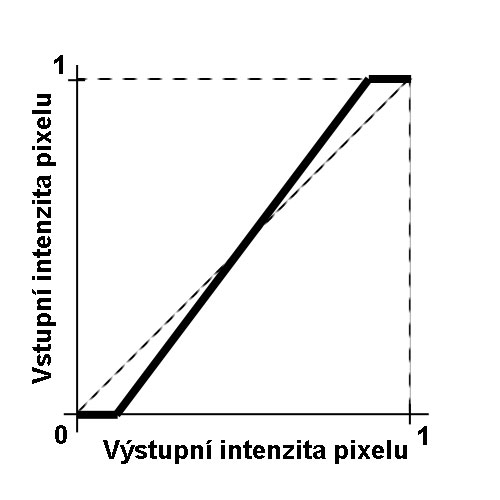
\includegraphics[width=0.3\textwidth,height=0.3\textwidth]{Text/IMG/Kontrast_Transformace_1.jpg}
		&\centering
			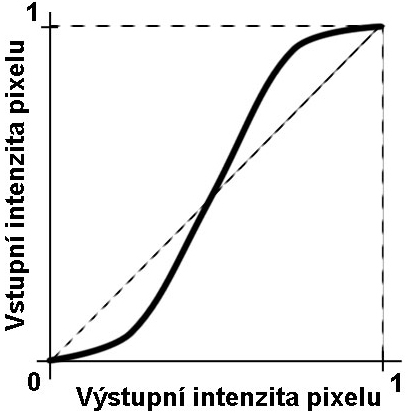
\includegraphics[width=0.3\textwidth,height=0.3\textwidth]{Text/IMG/Kontrast_Transformace_2.jpg}
		\end{tabular}
\end{table}





\subsection{Kontrast nelineárním způsobem}
S využitím jazyka Cg (případně C++ při odstranění OpenGL) lze implementovat nelineární změnu kontrastu zachovávající všechny informace v obrázku. V následující stati najdeme jednu z možných funkcí pro tuto transformaci.

Cílem je odvodit matematickou funkci, jejíž graf je podobný grafu \ref{table:kontrast} vpravo. Podobný průběh má funkce $tanh(c\cdot x)$ na intervalu $(-\infty,\infty)$, kde $c$ je parametr určující sklon křivky v bodě $0$. Funkce, kterou lze použít pro nelineární změnu kontrastu, musí navíc vyhovovat podmínkám: $f(\frac{1}{2})=\frac{1}{2}$, $f(0)=0$, $f(1)=1$. Odvoďme si přesný tvar takové funkce:

Graf funkce posuneme do bodu  $[\frac{1}{2},\frac{1}{2}]$:

\begin{equation}
f(x) = tanh(c\cdot(x-\frac{1}{2})) + \frac{1}{2}
\end{equation}

Omezíme obor hodnot na interval: $[0,1]$:

\begin{equation} \label{tanh1}
f(x) = \frac{1}{2}\cdot tanh(2\cdot c\cdot(x-\frac{1}{2})) + \frac{1}{2}
\end{equation}

Graf funkce (\ref{tanh1}) neprochází body $[0,0]$, $[1,1]$, to lze řešit různými úpravami. My přičteme k funkci (\ref{tanh1}) lineární funkci, která bude sloužit jako korekce:

\begin{equation}
f(x) = k\cdot(x-\frac{1}{2}) + \frac{1}{2}\cdot tanh(2\cdot c\cdot(x-\frac{1}{2})) + \frac{1}{2}
\end{equation}

Lze odvodit, že ke splnění podmínek: $f(0)=0$ a $f(1)=1$ je třeba aby:

\begin{equation}
k = 1 - tanh(c)
\end{equation}

Dosazením dostáváme výsledný tvar funkce:

\begin{center}
\framebox{ $f(x) = (1 - tanh(c))\cdot(x-\frac{1}{2}) + \frac{1}{2}\cdot tanh(2 \cdot c\cdot(x-\frac{1}{2})) + \frac{1}{2} $ }
\end{center}

Na grafech \ref{table:tanh} vidíme průběh nalezené funkce pro parametry $c=1$ a $c=2$.


\noindent
\begin{table}[ht]
	\captionsetup{tablename=Grafy}
	\caption{Graf nalezené funkce pro nelineární změnu kontrastu pro $c=1$ (vlevo) a $c=2$ (vpravo).}
	\label{table:tanh}
	\centering
		\begin{tabular}{p{0.3\textwidth}p{0.3\textwidth}}
			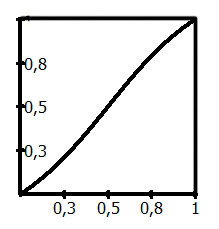
\includegraphics[width=0.3\textwidth,height=0.3\textwidth]{Text/IMG/nelinearni1.jpg}
		&
			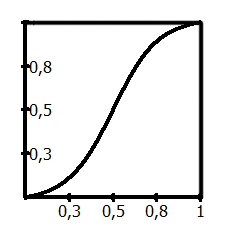
\includegraphics[width=0.3\textwidth,height=0.3\textwidth]{Text/IMG/nelinearni2.jpg}
		\end{tabular}
\end{table}


\newpage
\subsection{Kontrast a světlost v OpenGL}
Pro realizaci jednoduchých barevných transformací textury disponuje knihovna OpenGL funkcemi Bias a Scale.

\begin{itemize}
\item Voláním funkce Bias s parametry K,B provedeme přičtení konstanty K k hodnotě barevné složky B pro všechny pixely obrázku.
\item Voláním funkce Scale s parametry K,B provedeme vynásobení stávající barevné složky B konstantou K pro všechny pixely obrázku.
\end{itemize}

Transformační křivky obou funkcí vidíme na grafech \ref{table:biasscale}. Funkce Bias odpovídá změně jasu snímku. Změnu kontrastu musíme realizovat pomocí volání obou funkcí se správně dopočítanými parametry.

Pro změnu kontrastu voláme nejdřív funkci Scale s parametrem $s$, pak funkci Bias s parametrem $b$. Výsledek odpovídá lineární transformaci:
 
\framebox{ $ y = s \cdot x + b$ }

Vztah mezi parametry $b$ a $s$ takový, aby transformační křivka procházela bodem $[0.5,0.5]$, je:

\framebox{ $b=\frac{1}{2}\cdot(1-s)$ }

\noindent
\begin{table}[ht]
	\captionsetup{tablename=Grafy}
	\caption{Křivka transformací Bias (vlevo) a Scale (vpravo). Jejich správnou kombinací lze dosáhnout změny kontrastu.}
	\label{table:biasscale}
	\centering
		\begin{tabular}{p{0.35\textwidth}p{0.35\textwidth}}
			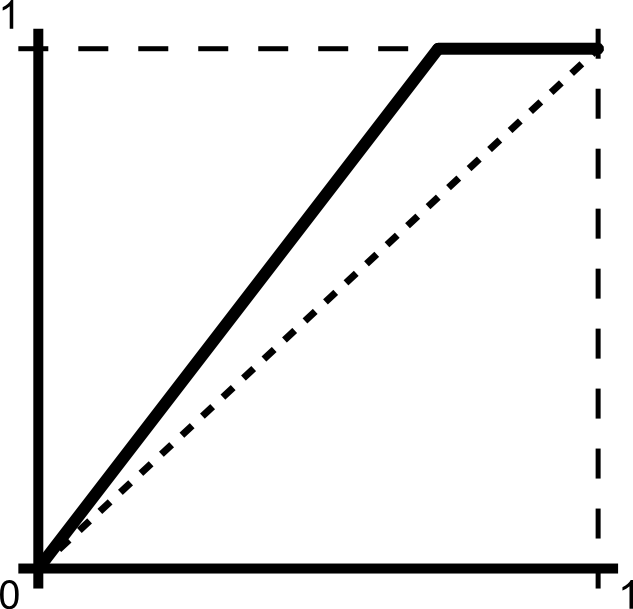
\includegraphics[width=0.3\textwidth]{Text/IMG/Bias.png}
		&
			\includegraphics[width=0.3\textwidth]{Text/IMG/Scale.png}
		\end{tabular}

\end{table}

\section{Rychlost vykreslování}
Jednou z otázek, na kterou se snaží najít odpověď tento VÚ, je to, zda by bylo možné z programu odstranit knihovny OpenGL a Cg toolkit. Knihovna OpenGL byla v programu použita pro zajištění plynulého provozu aplikace. Před odstraněním knihoven z programu musíme nejprve zjistit, zda bude možné realizovat zobrazování dodstatečně rychle i bez OpenGL. V takovém případě nebudeme už potřebovat ani Cg toolkit. 

Při vývoji DicomPresenteru byl kladen důraz na dostatečně plynulé ovládání. Pro práci s jakoukoliv aplikací je pohodlné, je-li mezi uživatelskou akcí a její realizací co nejkratší prodleva. V DicomPresenteru jsou výpočetně nejnáročnejčí akce: přesouvání snímků po obrazovce, úprava jasu a kontrastu snímků. Průměrný počet vykreslených snímků za sekundu při těchto akcích je při využití OpenGL 90 fps. Odhad toho, jak rychle poběží program bez OpenGL a Cg toolkit můžeme udělat tak, že naprogramujeme dvě aplikace, které budou mít na starosti pouze dvě zmiňované akce (posun snímku, změnu kontrastu). Jeden program bude využívat knihovny, druhý ne. Výkon testovacích aplikací a DicomPresenteru se bude značně lišit\footnote{Rozdíl v rychlosti vykreslování u DicomPresenteru a testovacích aplikací je způsoben tím, že DicomPresenter vedle vykreslování dat na obrazovku musí řešit další úlohy: zachytávání uživatelských akcí, předávání uživatelských akcí napříč objektovým modelem, vykreslování ovladacích prvků, vykreslování textů.}, ale z naměřených hodnot lze odhadnout, jak rychle poběží DicomPresenter bez OpenGL a Cg toolkit.

Uvažujme jednu z úloh a označme si:
\begin{itemize}
\item $fps_{lib}$ - počet naměřených snímků za sekundu v aplikaci využívající knihovny
\item $fps_{software}$ - počet naměřených fps v aplikaci nevyužívající grafické knihovny
\item $fps_{dp}$ - průměrný počet snímků kterého dosahuje DicomPresenter
\end{itemize}

Čas potřebný pro zpracování celého jednoho cyklu DicomPresenterem s OpenGL je:

\begin{equation}
t_{dp} = \frac{1}{fps_{dp}}
\end{equation}

Nahradíme-li vykreslování pomocí OpenGL softwarovým řešením problému, bude čas potřebný pro vykonání jednoho cyklu:

\begin{equation}
t_{software} = \frac{1}{fps_{dp}} - \frac{1}{fps_{lib}} + \frac{1}{fps_{software}}
\end{equation}

Průměrný počet snímků, kterého by měl dosahovat dicom presenter, je-li vykreslování realizováno softwarově, pak bude:

\begin{equation} \label{estimate}
fps_{odhad} = \left(\frac{1}{fps_{dp}} - \frac{1}{fps_{lib}} + \frac{1}{fps_{software}}\right)^{-1}
\end{equation}


\subsection{Změna kontrastu bez Cg toolkit}
Při programování změny kontrastu bez knihovny Cg toolkit se opíráme pouze o knihovnu Qt. Snímek máme v počítači uložen jako objekt třídy \clist{QImage}. Pro vyšší výkon nepoužíváme funkce knihovny Qt určené pro barevné transformace pixelů, ale měníme data přímo v paměti počítače pomocí pointerů. Díky těmto optimalizacím lze dosáhnout přibližně čtyřnásobného zvýšení výkonu, oproti použití k tomu určených funkcí Qt knihovny.

\begin{lstlisting}[label=DicomImageClass,caption={Změna kontrastu bez použití knihovny Cg toolkit.}]
for (int y = 0; y<h; y++){
	Rgb = (QRgb*)ShowImage.scanLine(y);
	for ( int x = 0; x < w; x++ ){
		Rgb[x] = qRgb(qRed(Rgb[x])*c+0.5*(1-c),qGreen(Rgb[x])*c+0.5*(1-c),qBlue(Rgb[x])*c+0.5*(1-c));
	}
}
\end{lstlisting}

\subsection{Změna kontrastu v Cg toolkit}

Knihovna Cg toolkit slouží dodatečným úpravám obrazu na grafické kartě. Pomocí Cg toolkit neměníme data uložená v paměti, ale přepočítáváme barevné hodnoty pixelů na výstupu. Pomocí příkazů knihovny Cg toolkit stačí aktivovat pixel shader před kreslením v OpenGL. Cg toolkit se pak postará o to, že na všechny pixely výstupu bude aplikována transformace popsaná v jazyce Cg (viz kód \ref{cg} ).

\begin{lstlisting}[label=cg,caption={Program v jazyce Cg pro změnu kontrastu snímku.}]
C3E3f_Output main(float2 texCoord :TEXCOORD0, uniform sampler2D decal :TEX0, uniform float contrast){
  C3E3f_Output OUT;
  OUT.color = tex2D(decal,texCoord)*contrast+0.5*(1-contrast);
  return OUT;
}
\end{lstlisting}

\subsection{Posun snímku bez OpenGL}
V případě posunutí snímku bez OpenGL postupujeme podobně jako při změně kontrastu. V porovnání se změnou kontrastu máme ale v programu dva objekty typu QImage. Jeden reprezentuje pracovní plochu, druhý reprezentuje zobrazovaný snímek. Když chceme vykreslit snímek na obrazovku, nejprve vynulujeme všechna data v pracovní ploše a pak zkopírujeme data ze snímku na požadované místo na pracovní ploše.

Podobně jako v prvním příkladě této kapitoly není možné pro tuto úlohu použít předem připravené fukce Qt knihovny, neboť je pak úloha násobně pomalejší.

\begin{lstlisting}[caption={Funkce pro vykreslení snímku na zadanou pozici napsaná bez použití OpenGL.}]
void Workspace::draw(QPoint leftTop, QImage *sourceImage){
	for ( int y = 0; y < this->height(); y++ ){
		QRgb *workspaceImageLinePtr = (QRgb*)this->scanLine(y);
		for ( int x = 0; x < this->width(); x++ ){
			workspaceImageLinePtr[x] = qRgb(0,0,0);
		}
	}
	for ( int y = 0; y < sourceImage->height(); y++ ){
		QRgb *sourceImageLinePtr = (QRgb*)sourceImage->scanLine(y);
		QRgb *workspaceImageLinePtr = (QRgb*)this->scanLine(leftTop.y() + y);
		for ( int x = 0; x < sourceImage->width(); x++ ){
			workspaceImageLinePtr[leftTop.x() + x] = qRgb(qRed(sourceImageLinePtr[x]),qGreen(sourceImageLinePtr[x]),qBlue(sourceImageLinePtr[x]));
		}
	}
}
\end{lstlisting}


\subsection{Posun snímku s OpenGL}

Realizovat posunutí snímku pomocí OpenGL je výrazně jednodušší. Pomocí přibližně desítky příkazů OpenGL popíšeme co a kam chceme zobrazit. OpenGL za nás pak řeší např. otazky přepočítávání rozměrů při zvětšení a zmenšení okna.

\begin{lstlisting}[caption={Funkce pro vykreslení snímku využívající OpenGL.}]
void GLPainter::Paint(int translationX){
	glClear(GL_COLOR_BUFFER_BIT);
	float ratio = (float)translationX/im->width().;
	glBegin(GL_POLYGON);
		glColor3f (Brightness, Brightness, Brightness);
		glTexCoord3f(0.,0.,0.);	glVertex2f(ratio+ -1.,-1.);
		glTexCoord3f(0.,1.,0.);	glVertex2f(ratio+ -1., 1.);
		glTexCoord3f(1.,1.,0.);	glVertex2f(ratio+  0., 1.);
		glTexCoord3f(1.,0.,0.);	glVertex2f(ratio+  0.,-1.);
	glEnd();
}
\end{lstlisting}




\subsection{Naměřené hodnoty}

Výsledky získane z testovacích aplikací jsou vidět v tabulce \ref{vysledky}. Daná úloha je vždy pomocí knihoven OpenGL, respektive Cg řešena přibližně šestkrát rychleji. Použijeme-li vzoreček (\ref{estimate}), pak lze spočítat, že změna kontrastu by v hotové aplikaci měla probíhat s rychlostí nejméně 36ti snímků za sekundu a posun snímku by měl běžet nejhůře s 48mi snímky za sekundu. Tato rychlost je dostačující pro použití programu. OpenGL z aplikace tedy lze odstranit.

\noindent
\begin{table}[ht]
	\caption{Počty snímků za sekundu, kterých bylo dosaženo v testovacích aplikacích.}
  \label{vysledky}
	\centering
\begin{tabular}{| p{5cm} | l | l | l | }

  \hline                       
  Úloha & Požité knihovny & Snímků za vteřinu \\
  \hline
  \hline
  Změna kontrastu & Qt &  90 fps\\
  \hline
  Změna kontrastu & Qt, OpenGL, Cg & 600 fps\\
  \hline
  Posun snímku & Qt & 50  fps \\
  \hline
  Posun snímku  & Qt, OpenGL & 250 fps \\
  \hline  
\end{tabular}

\end{table}
